\section{Performance Results} % what is the problem. what is our solution.

Figure \ref{fig:compare} shows the predicted time from all algorithms except for KCCA. All three of them have the same trend of performance among both kernels, with Random Forest fits best, and Boosted Regression Tree fits decently. The magenta dots on both subfigures (a) and (b) are the lines for Kernel Ridge Regressions. Its predicted time really fluctuates between being on the correct running time, in the middle under the curve, and on zero lines. I had to plot them as dots or we would get a big thick zigzag and wouldn't be able to see other lines.

It is worth noting that the irregular spike the Random Forest algorithm experienced in Figure \ref{fig:compare}(b) might also be experienced by Boosted Regression Tree as well, although less much noticable, while it doesn't affect Kernel Ridge Regression. This should be some tree-specific error.

\begin{figure*}[h]
  \centering
  \begin{subfigure}[b]{0.8\textwidth}
    \centering
    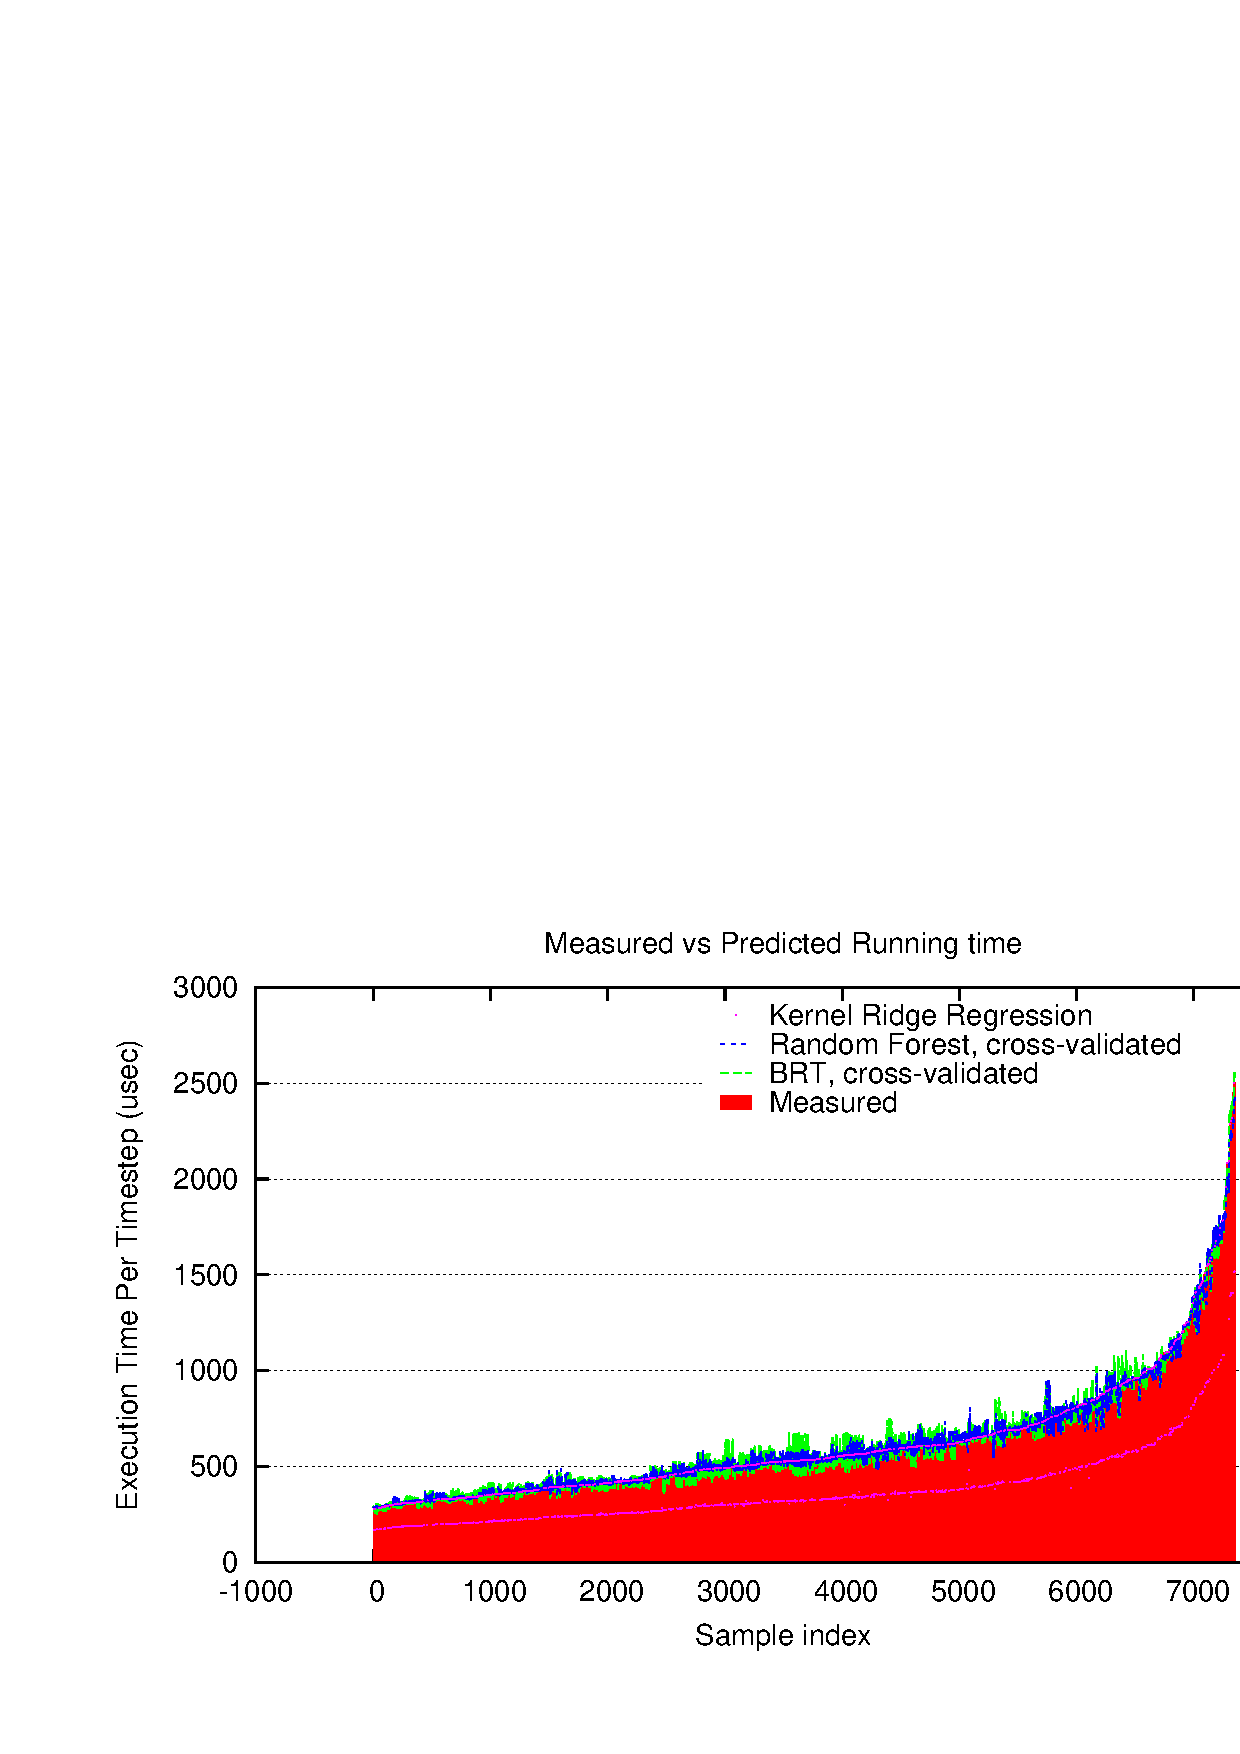
\includegraphics[width=\textwidth]{images/simple-cmp}
    \caption{Simple Stencil}
    \label{fig:simple-compare}
  \end{subfigure}
	%
  ~ %add desired spacing between images, e. g. ~, \quad, \qquad etc.
    %(or a blank line to force the subfigure onto a new line)
  \begin{subfigure}[b]{0.8\textwidth}
    \centering
    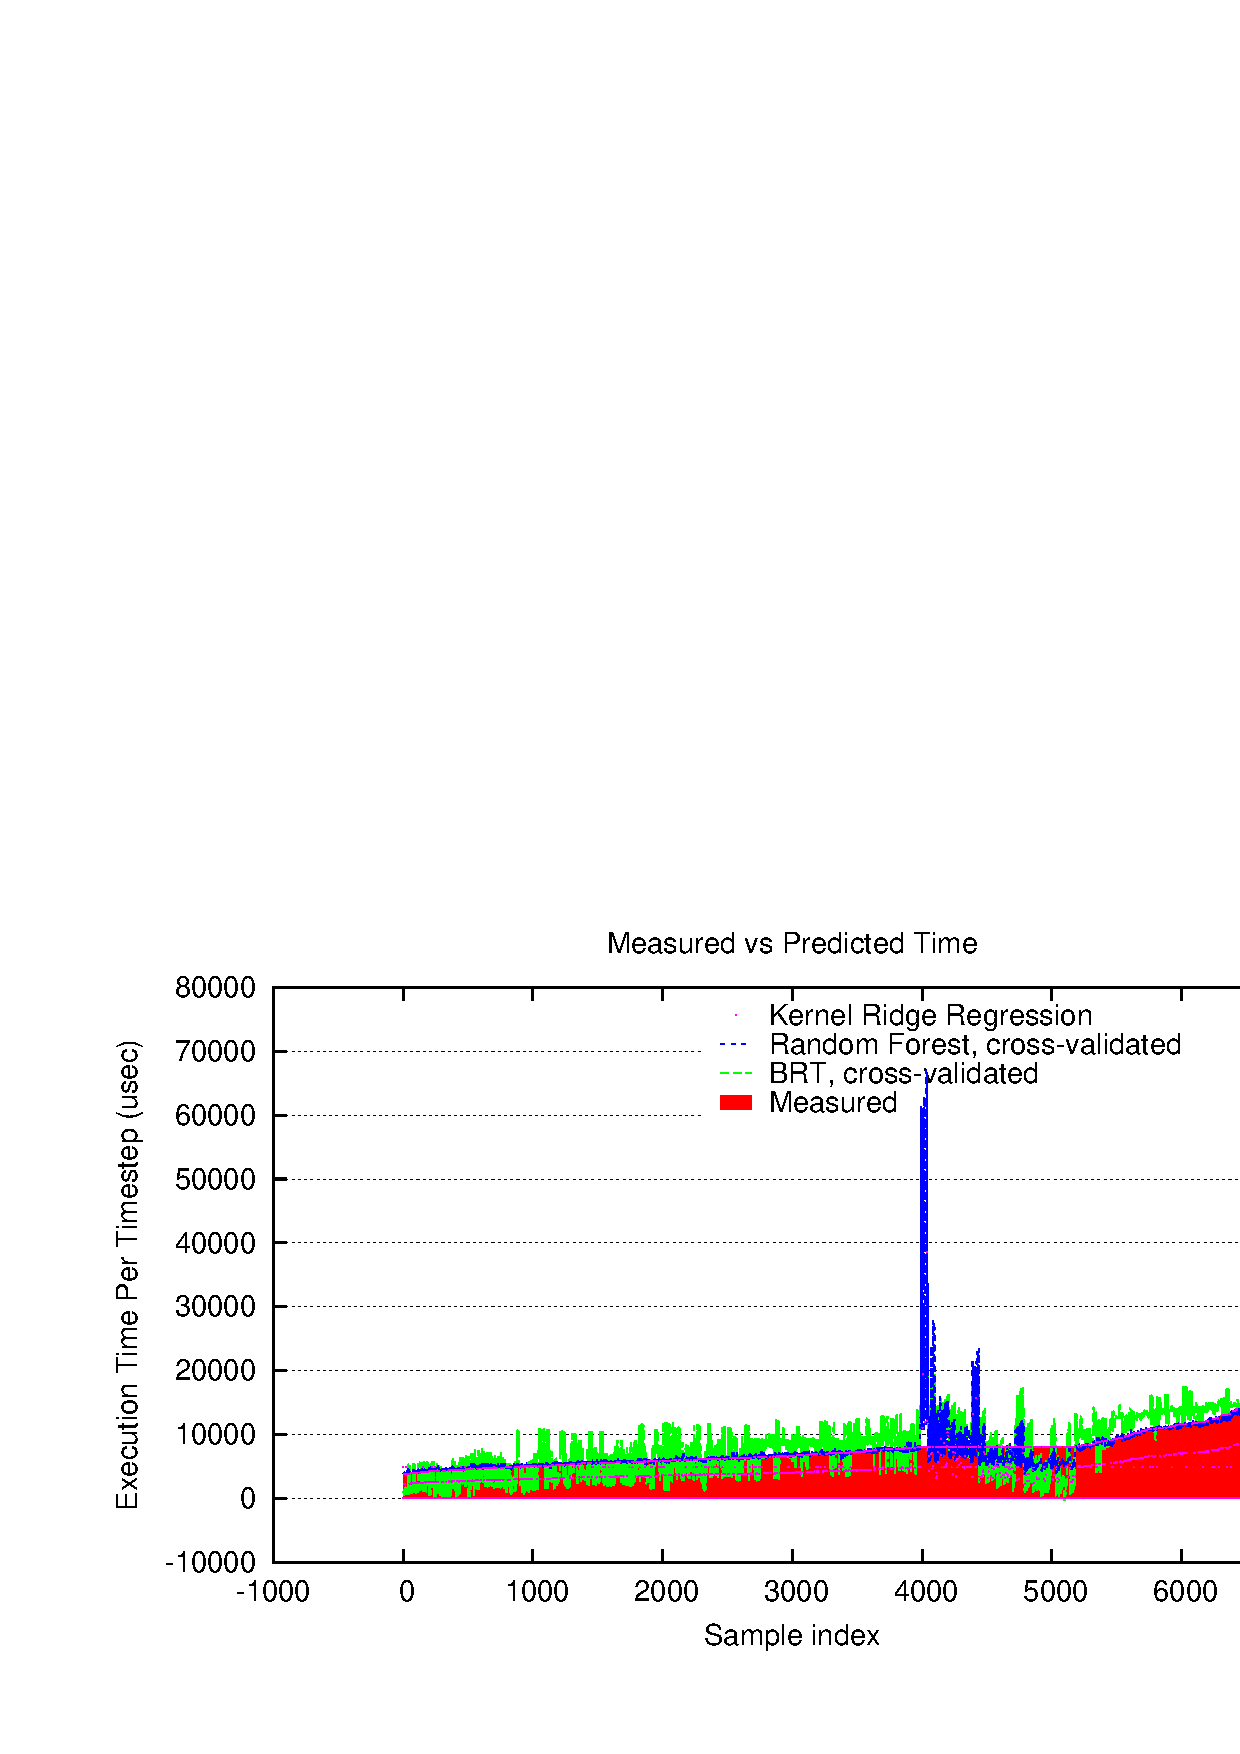
\includegraphics[width=\textwidth]{images/hypterm-cmp}
    \caption{Hypterm Kernel}
    \label{fig:hypterm-compare}
  \end{subfigure}
  \caption{Comparision of predicted results of Gradient Boosted Regression Tree, Kernel Ridge Regression, and Random Forest.}
\label{fig:compare}
\end{figure*}

Now let us proceed to see how well they are in action. I use Hill-Climbing algorithm for 75 iterations to search for best configurations for Gradient Boosted Regression Tree, Random Forest, and Kernel Ridge Regression. And use the same genetic algorithm with KCCA as Ganapathi et al.\ Table \ref{table:simple} and Table \ref{table:hypterm} shows the best running time of all the machine learning algorithms in Simple Stencil and Hypterm kernel, respectively. The columns are arranged from worst to best performance. The average running time comparison plot is also shown in Figure \ref{compare_all}. KCCA is in a league of its own, with the average case 0.1\% away from the best configurations in simple stencil and 0.3\% in Hypterm kernel. Random Forest is the second best despite its spike. Gradient Boosted Regression Tree does hold itself. Kernel Ridge Regression tree lagging behind so badly is not very surprising considering the model is quite simple. However, this might also be me choosing wrong kernel too.

Other factor to be concern is time, however, in this project the largest number of training set is 1000, at which even KCCA takes about the same time as other algorithms. How we would tradeoff the tuning ability with time would be an interesting topic to be explore later. The tree algorithms also perform better when having more number of samples. But as of now if we have around thousands of sample, I would definitely choose KCCA, then Random Forest, and then Boosted Regression Tree.

\begin{table}[h]
\caption{Simple Stencil Kernel Tuning Results (Time in Microseconds)}
\center
\begin{tabular}{r c c c c}
\hline
 & KRR	& GBRT	& Random Forest	& KCCA \\
\hline\hline
Average	& 684.4274	& 318.0251	& 302.9823	& 275.5940 \\
Minimum	& 277.1379	& 276.9882	& 275.3037	& 275.3037 \\
Maximum	& 1958.7149	& 396.7846	& 324.7757	& 276.9702 \\
Standard Deviation	& 296.2554	& 20.0290	& 15.1782	& 0.5464 \\
\% error of Average from Optimal	& 148.6082	& 15.5179	& 10.0538	& 0.1054 \\
\hline
\label{tbl:simple}
\end{tabular}
\label{table:simple}
\end{table}

\begin{table}[h]
\caption{Hypterm Kernel Tuning Results (Time in Microseconds)}
\center
\begin{tabular}{r c c c c}
\hline
 & KRR	& GBRT	& Random Forest	& KCCA \\
\hline\hline
Average	& 6927.8448	& 4412.7641	& 4088.5444	& 3723.5620 \\
Minimum	& 3770.1504	& 3715.6557	& 3711.3638	& 3715.6557 \\
Maximum	& 73002.4738	& 8037.9917	& 8037.9917	& 3764.0666 \\
Standard Deviation	& 4520.2231	& 1084.9311	& 635.4020	& 17.1137 \\
\% error of Average from Optimal	& 86.6657	& 18.8987	& 10.1629	& 0.3287 \\
\hline
\label{tbl:hypterm}
\end{tabular}
\label{table:simple}
\end{table}

\begin{figure*}[h]
\centering
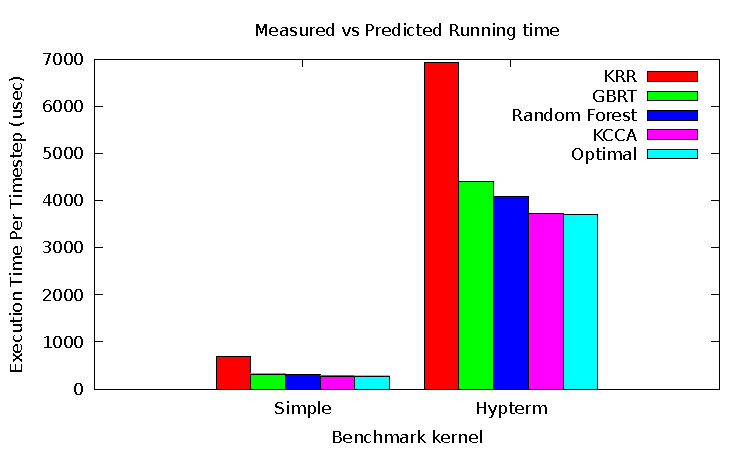
\includegraphics[width=0.8\textwidth]{./images/compare_all.pdf}
\caption{Comparison of all machine learning methods on both simple stencil and Hypterm kernels}
\label{fig:compare_all}
\end{figure*}
